\documentclass[11pt,a4paper]{article}

\usepackage[margin=2.5cm]{geometry}
\usepackage[T1]{fontenc}
\usepackage{lmodern}
\usepackage{graphicx}
\usepackage{booktabs}
\usepackage{float}
\usepackage{xcolor}
\usepackage{hyperref}
\usepackage{caption}

\hypersetup{colorlinks=true, linkcolor=blue!50!black, urlcolor=blue!50!black}
\graphicspath{{figures/}{../figures/}}   % works in Overleaf (figures/) and in the repo (../figures/)

% Red marker for anything a teammate still has to fill in. Search for TODO before submitting.
\newcommand{\todo}[1]{\textcolor{red}{[TODO: #1]}}

\title{SunCast: Forecasting Rooftop Solar Output and Savings in Pakistan\\
\large Deliverable 1: Problem Definition and Data Pipeline}
\author{Anoosha Rizwan Vohra (24L-3096) \and Kainat Afzal (24L-3084) \and Manumha Nadeem (24L-3097)}
\date{\today}

\begin{document}
\maketitle
\tableofcontents
\newpage

\section{Introduction}
Rooftop solar has become one of the most talked about ways for households in Pakistan to deal with rising electricity bills. Installing a system is a large investment, but most people decide with little more than a salesperson's estimate or an online calculator that uses yearly averages. Those estimates ignore the things that actually change how much power panels produce from day to day, such as clouds, smog, heat, and the climate of each city.
 
 SunCast is a web application that aims to close this gap. A user enters their city, the size of their solar system, and their electricity tariff, and the app forecasts how much power the system will generate over the next few days using live weather data and a machine learning model. The forecast is converted into estimated savings in rupees, and a chatbot answers common solar questions and suggests retailers in the user's city.
 
This report covers the first deliverable of the project: defining the problem and building the data pipeline. Section 2 and Section 3 describe the problem and who the app is for, and Section 4 explains why machine learning is needed. Sections 5 to 7 describe how we collected, cleaned, and prepared the data, and Section 8 presents our exploratory analysis. Section 9 outlines the next steps.
 

\section{Problem Statement}

Electricity prices in Pakistan have gone up sharply over the last few years, and for many households the monthly bill has become one of their biggest expenses. Because of this, more and more people are looking at rooftop solar as a way to cut costs. The problem is that installing solar is a big financial decision, and most people make it with very little reliable information about what the system will actually do for them.
 
Most solar calculators available online work with yearly averages. They take the size of the system, multiply it by an average amount of sunlight for the region, and give a single number. This approach misses several things that have a real effect on how much power panels produce in Pakistan:
 
\begin{itemize}
    \item \textbf{Clouds and weather:} output changes a lot from day to day, and a yearly average says nothing about what to expect this week.
    \item \textbf{Smog and dust:} in cities like Lahore, winter smog blocks a noticeable share of sunlight for weeks at a time, which simple calculators ignore completely.
    \item \textbf{Heat:} solar panels become less efficient as they get hotter, so the hottest months do not produce as much as the strong sunlight would suggest.
    \item \textbf{Location:} sunlight and weather patterns differ between cities like Karachi, Lahore, and Peshawar, but many tools treat the whole country the same way.
\end{itemize}
 
This creates two problems. People who are thinking about buying solar cannot tell how much they will really save or whether the investment is worth it. People who already have solar cannot tell whether their system is performing as it should, or plan their electricity use around the days and hours when generation will be high.
 
On top of this, the practical information people need is scattered. Common questions about inverter types, whether a battery is worth the cost, how net metering works, and which retailers in their city are trustworthy are usually answered through word of mouth or sales pitches, which may not be accurate or unbiased.
 
SunCast addresses these problems with a web application that forecasts solar generation for a specific location using live weather data and a machine learning model trained on historical sunlight, weather, and air quality data. The forecast is converted into estimated savings in rupees, and a built in chatbot answers common solar questions and suggests retailers in the user's city.


\section{Target Audience}

SunCast is designed for the following groups of users:
 
\begin{itemize}
    \item \textbf{Homeowners considering solar:} people who want to know how much a system of a given size would generate at their location and how much money it would save before they spend on an installation.
    \item \textbf{Existing solar owners:} people who already have panels and want to know what to expect over the next few days, check whether their system is performing normally, and plan heavy electricity use (such as running air conditioners, washing machines, or water pumps) for high generation hours.
    \item \textbf{Small businesses:} shops, clinics, schools, and offices that run during daytime hours and want to understand how much of their electricity demand solar could cover.
    \item \textbf{First time buyers with little technical knowledge:} users who do not understand terms like inverter capacity or net metering and need simple, trustworthy answers before talking to a retailer.
\end{itemize}
 
For the first version, the app covers five major cities: Lahore, Karachi, Islamabad, Peshawar, and Multan. These cities were chosen because they cover different climates across the country, from the humid coastal weather of Karachi to the smoggy winters of Lahore and the hotter, drier conditions of Multan. The system is built so that more cities can be added later by including their coordinates in the data pipeline.


\section{AI Justification}
Solar output depends on many factors that affect each other in complicated,
nonlinear ways: cloud cover, smog and dust that block sunlight, panels losing
efficiency when they get hot, and changes between seasons. Our analysis
supports this: sunlight varies strongly by month and city, and cloud cover
and PM2.5 each reduce it. A fixed formula or rule-based program uses fixed
averages, so it cannot capture these effects together. A machine learning
model can learn them directly from real data and give a more accurate
forecast for each city.

The chatbot also needs AI. People ask solar questions (inverters, batteries,
net metering) in plain, everyday language, and rule-based code cannot handle
so many different ways of asking the same question.

\section{Data Collection}
\label{sec:collection}

SunCast needs three kinds of data: weather and sunlight for Pakistani cities, smog, and real solar panel output. Four sources cover them (Table~\ref{tab:sources}). All collection code is in the \texttt{data\_scripts/} folder of our repository, and the scripts write log files that we kept as evidence of each download.

\begin{table}[H]
\centering
\small
\begin{tabular}{p{3.1cm} p{4.0cm} p{2.9cm} p{3.4cm}}
\toprule
\textbf{Source} & \textbf{What it gives us} & \textbf{How we got it} & \textbf{Script} \\
\midrule
NASA POWER hourly API & Sunlight (W/m$^2$), temperature, humidity, wind speed & API, no key needed & \texttt{fetch\_nasa\_\allowbreak power.py} \\
Open-Meteo Historical Weather API & Cloud cover (\%) & API, no key needed & \texttt{fetch\_\allowbreak openmeteo.py} \\
Open-Meteo Air Quality API & PM2.5 ($\mu$g/m$^3$), our measure of smog & API, no key needed & \texttt{fetch\_\allowbreak openmeteo.py} \\
Kaggle ``Solar Power Generation Data'' & Real power output of a solar plant, with its own weather sensor readings & Download from Kaggle & \texttt{load\_kaggle\_\allowbreak generation.py} \\
Retailer list & Solar retailers by city & Compiled by hand by the team & \texttt{data/retailers.csv} \\
\bottomrule
\end{tabular}
\caption{Data sources used in SunCast.}
\label{tab:sources}
\end{table}

\subsection{Study area and period}
We collected data for five cities that together cover very different climates: Lahore, Karachi, Islamabad, Peshawar and Multan. Each city is represented by one coordinate point, and all APIs were queried for the same points. We used the full year 2024, hourly, which gives $5 \times 8{,}784 = 43{,}920$ hourly records (2024 was a leap year).

\subsection{NASA POWER (sunlight, temperature, humidity, wind)}
\texttt{fetch\_nasa\_power.py} requests four variables from the NASA POWER hourly point API with the renewable energy community setting: all-sky surface sunlight (\texttt{ALLSKY\_SFC\_SW\_DWN}, which already accounts for clouds), air temperature at 2~m, relative humidity at 2~m and wind speed at 10~m. The script asks for one month at a time for each city, retries a request up to three times if it fails, and pauses one second between requests to avoid overloading the service. NASA returns times in UTC, so the script converts them to Pakistan time (Asia/Karachi) before saving. Missing readings are marked with the code $-999$ in the API output, and our cleaning step replaces them (see the Data Cleaning section). The log (\texttt{data\_scripts/logs/fetch\_nasa\_power.log}) records every request: all 12 months were downloaded for all 5 cities, giving 8{,}784 rows per city.

\subsection{Open-Meteo (cloud cover and smog)}
NASA POWER does not give cloud cover or air quality, so \texttt{fetch\_openmeteo.py} adds them from two Open-Meteo APIs: the Historical Weather API for hourly cloud cover, and the Air Quality API for hourly PM2.5. Both are requested in the Asia/Karachi time zone so their timestamps line up with the NASA data. Because the NASA times were shifted from UTC to Pakistan time (five hours ahead), the last hours of December 2024 fall on 1 January 2025. The script therefore asks for one extra day, which is why each city has 8{,}808 Open-Meteo rows (366 days plus one extra day). Table~\ref{tab:evidence} summarises the evidence from the log files.

\begin{table}[H]
\centering
\small
\begin{tabular}{p{5.0cm} p{2.4cm} p{4.8cm}}
\toprule
\textbf{Step} & \textbf{Rows} & \textbf{Log file} \\
\midrule
NASA POWER, per city & 8{,}784 & \texttt{fetch\_nasa\_power.log} \\
NASA POWER, five cities, cleaned & 43{,}920 & \texttt{clean\_nasa\_report.txt} \\
Open-Meteo, per city & 8{,}808 & \texttt{fetch\_openmeteo.log} \\
After merge with NASA data & 43{,}920 & \texttt{fetch\_openmeteo.log} \\
Missing cloud cover / PM2.5 after merge & 0 / 0 & \texttt{fetch\_openmeteo.log} \\
\bottomrule
\end{tabular}
\caption{Row counts recorded by the collection scripts.}
\label{tab:evidence}
\end{table}

\subsection{Merging weather sources}
The NASA data and the Open-Meteo data are joined on city and timestamp. We used a left join so that every NASA row is kept, and added cloud cover and PM2.5 where the timestamps match. All 43{,}920 rows matched, with no missing cloud cover or PM2.5 values. The script also checks that cloud cover stays between 0 and 100\% and that PM2.5 is not negative (any invalid value would be set to missing and filled only if the gap is three hours or shorter), but no value needed fixing. The script saves two versions of the merged table:
\begin{itemize}
  \item \texttt{merged\_weather.csv}, which keeps the city name, used for exploratory analysis;
  \item \texttt{merged\_weather\_encoded.csv}, where the city column is one hot encoded into five 0/1 columns (\texttt{city\_Lahore}, \texttt{city\_Karachi}, and so on), used for modelling.
\end{itemize}

\subsection{Kaggle solar plant data}
Weather data alone cannot tell us how much power a panel produces, so we need a measured output as the training target. We use the public Kaggle dataset \emph{Solar Power Generation Data} by Ani Kannal (\url{https://www.kaggle.com/datasets/anikannal/solar-power-generation-data}). It contains two files for one solar plant: \texttt{Plant\_1\_Generation\_Data.csv} (power output of each inverter, recorded every 15 minutes) and \texttt{Plant\_1\_Weather\_Sensor\_Data.csv} (sunlight, ambient and module temperature measured at the plant). The Kaggle data comes from a plant in India in 2020 and the file has no city column, so it is used to learn how weather turns into power, while the city-specific weather features come from NASA POWER and Open-Meteo. \texttt{load\_kaggle\_generation.py} loads both files and prints their shapes.

\subsection{Retailer list}
For the app's retailer suggestions we compiled a directory of 39 solar retailers and installers across the five study cities (8 in Lahore, 8 in Karachi, 8 in Islamabad, 7 in Peshawar and 8 in Multan). Each entry has four columns: name, area, contact and rating. Business names, areas, phone numbers and customer ratings were collected by hand from public Google Maps listings in October 2026. The directory is stored in \texttt{data/retailers.csv} and will be used by the web app to suggest local retailers to users.

\subsection{Reproducibility}
Large data files are not stored in the repository (they are excluded by \texttt{.gitignore}). Anyone can recreate them by running the scripts in this order: \texttt{fetch\_nasa\_power.py}, \texttt{clean\_nasa.py}, \texttt{fetch\_openmeteo.py}. The repository is at \url{https://github.com/anushavohra/suncast}, and a link to the cleaned NASA data is in the README.

\section{Data Cleaning}

We cleaned two datasets: the NASA POWER weather data (\texttt{clean\_nasa.py}) and the Kaggle solar plant data (\texttt{clean\_generation.py}). The Open-Meteo values were validated during the merge, as described in the Data Collection section. Each script prints a before and after summary, and the NASA script saves it to \texttt{data\_scripts/logs/clean\_nasa\_report.txt}.
 
\subsection{NASA POWER weather data}
 
\texttt{clean\_nasa.py} combines the hourly files for all five cities into one table, renames the NASA variable codes to readable names (irradiance, temperature, humidity, and wind speed), and applies the following steps:
 
\begin{itemize}
    \item \textbf{Missing values:} NASA POWER marks missing readings with the code $-999$. These are replaced with empty values, and gaps of up to three hours are filled by time based interpolation, one city at a time so cities never mix. Longer gaps are dropped.
    \item \textbf{Duplicates:} rows with the same city and timestamp are removed.
    \item \textbf{Impossible values:} negative irradiance, and any irradiance between 21:00 and 04:00 when the sun is always down, are set to zero. Irradiance above the solar constant (about 1361 W/m$^2$), temperature outside $-20$ to $55\,^{\circ}$C, humidity outside 0 to 100\%, and wind speed outside 0 to 40 m/s are treated as errors.
    \item \textbf{Statistical outliers:} values more than 1.5 times the interquartile range beyond the quartiles are counted but kept, because heatwaves and windy days are real weather that the model needs to learn from.
\end{itemize}
 
Table~\ref{tab:nasa_cleaning} shows the results. The 2024 NASA POWER data passed every check, with no missing values, duplicates, or physically impossible readings, which confirms it as a reliable source. The only notable finding was 1,931 statistical outliers in wind speed. Wind speed is usually low with occasional strong gusts, so the interquartile range rule flags many real windy and stormy hours; we kept them on purpose.
 
\begin{table}[h]
\centering
\begin{tabular}{lr}
\hline
\textbf{Check} & \textbf{Count} \\
\hline
Rows before cleaning & 43,920 \\
Missing values (all four columns) & 0 \\
Duplicate rows removed & 0 \\
Impossible values fixed & 0 \\
Wind speed outliers (kept) & 1,931 \\
Temperature and humidity outliers & 0 \\
Rows after cleaning & 43,920 \\
\hline
\end{tabular}
\caption{Results of cleaning the NASA POWER data (five cities, 2024).}
\label{tab:nasa_cleaning}
\end{table}
 
Claude finished the response

\subsection{Kaggle plant data}
\texttt{clean\_generation.py} cleans the Kaggle plant data and merges the
generation file with the weather sensor file on the timestamp.
\begin{itemize}
  \item Missing values: none found.
  \item Duplicate rows (same timestamp and inverter): none found.
  \item Negative power values: none found.
  \item Merge with the sensor data: 68,778 rows became 68,774 rows,
        because 4 generation rows had no matching sensor reading.
  \item Inverter faults: 63 rows where sunlight was present
        (irradiation above 0.2) but the inverter output was zero were
        removed as outliers.
  \item Night readings: no rows had sunlight above zero at night.
\end{itemize}
The cleaned Kaggle table has 68,711 rows.

\section{Feature Strategy}
\texttt{feature\_engineering.py} prepares the cleaned Kaggle table for
modelling.
\begin{itemize}
  \item \textbf{Sine/cosine encoding} of hour and month, because time is a
        cycle (hour 23 is close to hour 0, and December is close to January).
  \item \textbf{One hot encoding} of the inverter ID (22 inverters).
        The city is one hot encoded separately in the merged weather table
        (see the Data Collection section), because the Kaggle data has no
        city column.
  \item \textbf{StandardScaler} on ambient temperature, module temperature
        and irradiation, so that all inputs have mean 0 and standard
        deviation 1. DC and AC power are the targets, so they are not scaled.
  \item \texttt{DAILY\_YIELD} and \texttt{TOTAL\_YIELD} were removed because
        they already contain the power result and would let the model cheat.
\end{itemize}
The final feature table has 68,711 rows and 31 columns.

\section{Exploratory Data Analysis}
\label{sec:eda}

Before building any model we looked at the data to check that it behaves the way physics says it should, and to find which inputs matter. All charts are produced by \texttt{data\_scripts/eda.py} from the merged weather table (43{,}920 hourly rows, five cities, 2024) and from the cleaned Kaggle plant data.

\subsection{Sunlight by month and city}
Figure~\ref{fig:month} shows the average daily sunlight energy for each month. All five cities follow the same shape: sunlight rises from winter to a peak in May or June, then falls again. The peak is between 7.2 and 7.5~kWh/m$^2$/day for every city (May for Islamabad, Karachi, Lahore and Multan, June for Peshawar).

The cities differ most in winter and during the monsoon. Lahore and Multan fall to about 1.7 and 1.9~kWh/m$^2$/day in January, roughly a quarter of their May values. This is consistent with winter fog and smog in the Punjab, although this chart alone does not prove the cause. Karachi stays much more even through the year; its lowest month is August (4.1~kWh/m$^2$/day), which fits the cloudy monsoon season. Over the full year, Karachi receives the most sunlight (5.31~kWh/m$^2$/day), followed by Peshawar (5.06), Islamabad (4.80), Multan (4.77) and Lahore (4.72). Two points matter for the product: location and season change the expected output a lot, so a single fixed average cannot be right for every user, and the winter dip in Lahore and Multan is exactly the kind of effect a data-driven model should capture.

\begin{figure}[H]
\centering
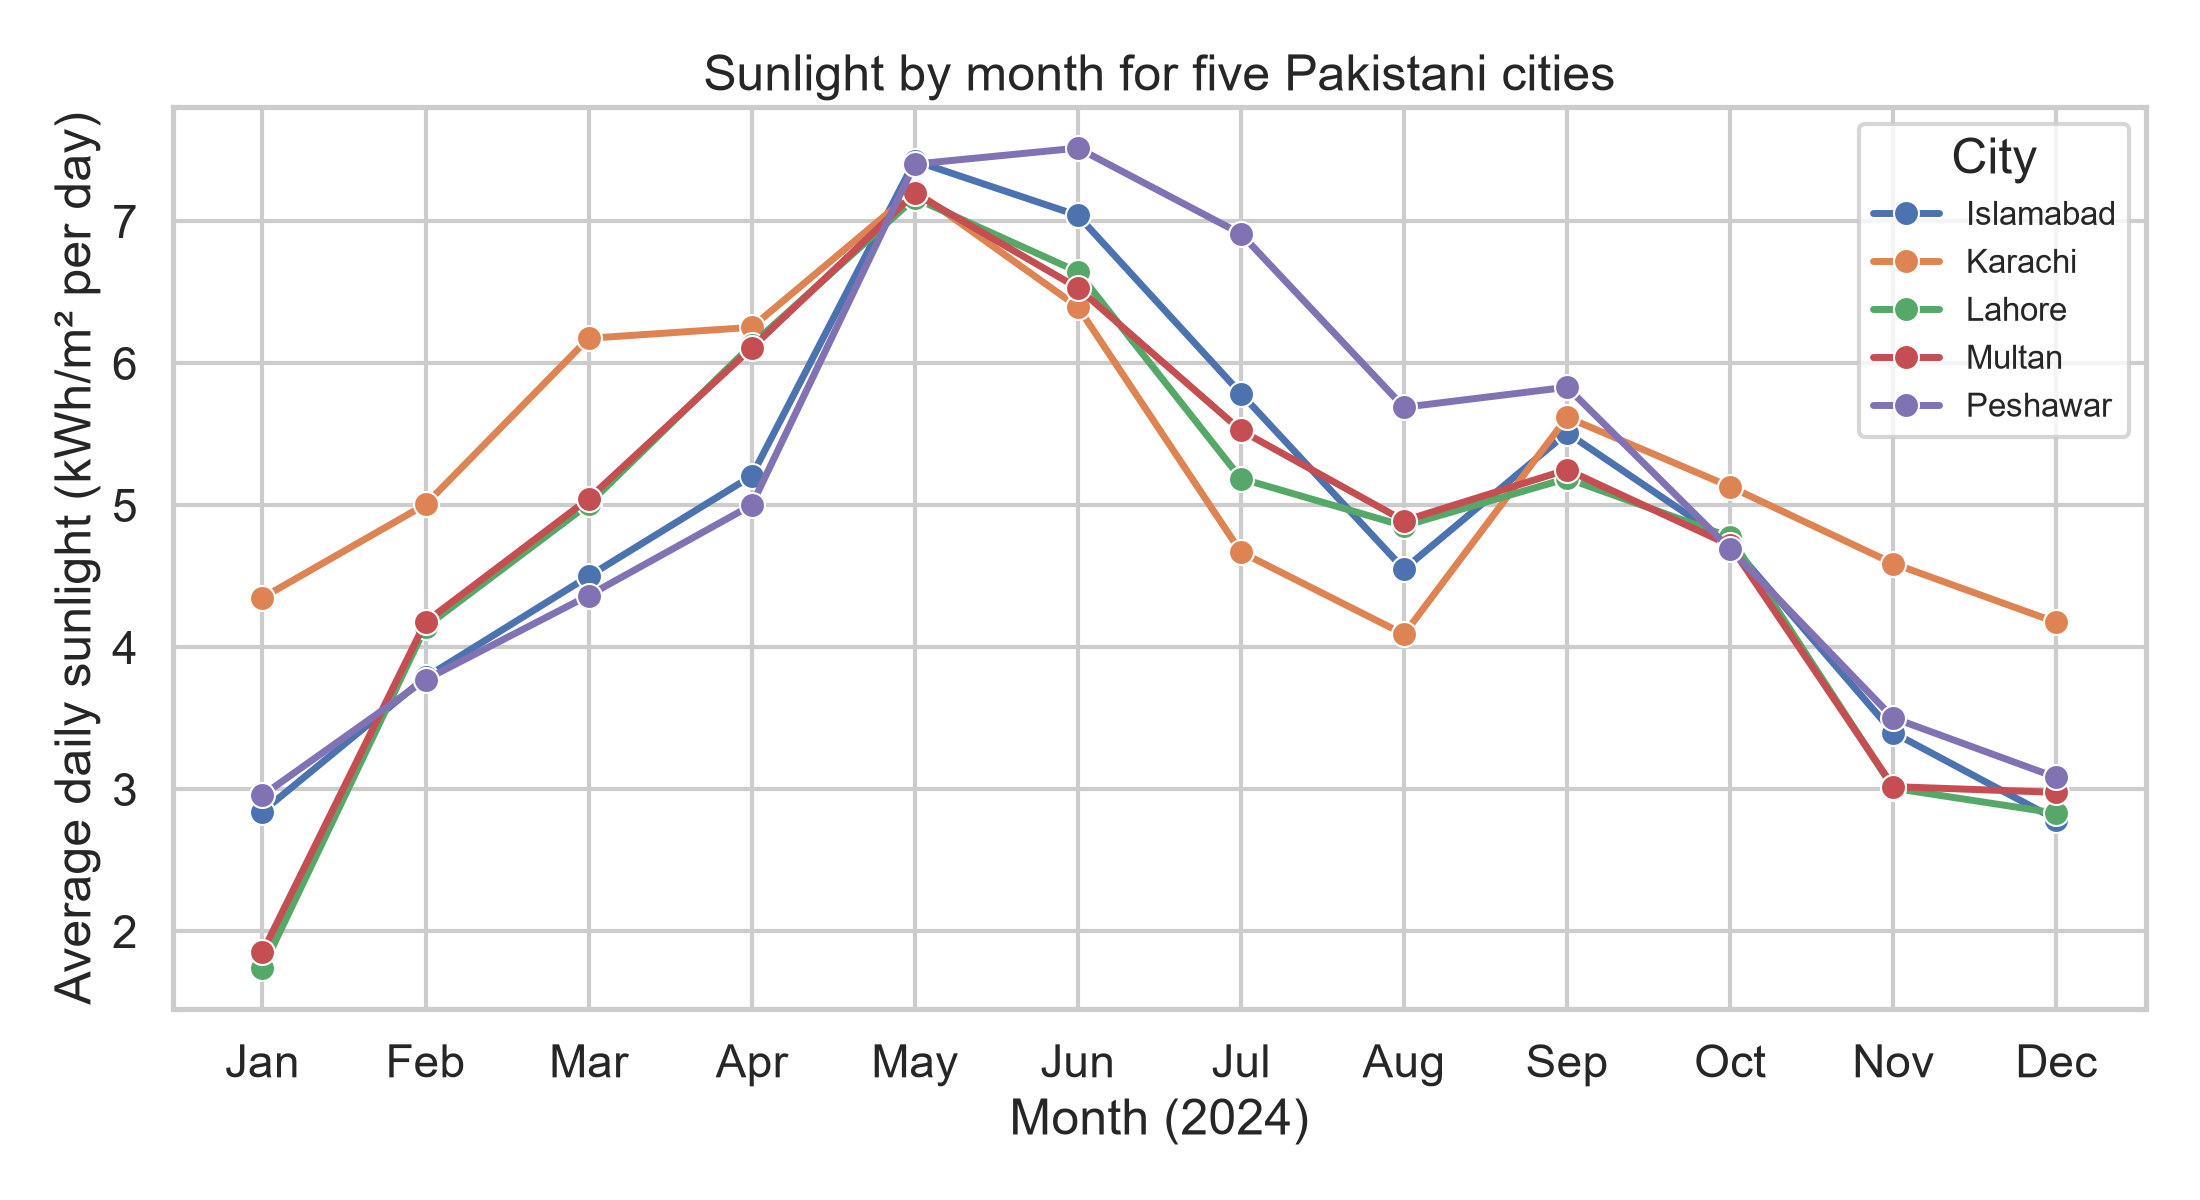
\includegraphics[width=0.88\textwidth]{01_sunlight_by_month.png}
\caption{Average daily sunlight energy by month for the five cities (2024, NASA POWER).}
\label{fig:month}
\end{figure}

\subsection{Correlation between weather features}
Figure~\ref{fig:corr} shows how the weather variables relate to each other during daytime hours (night hours are excluded, because sunlight is always zero then and would distort the picture). Sunlight is positively related to temperature ($r = 0.45$) and negatively related to humidity ($r = -0.42$): sunny hours are warmer and drier. Cloud cover and PM2.5 both reduce sunlight, but only mildly in this hour-by-hour view ($r = -0.20$ and $r = -0.18$). These links look weak because each hourly value also depends on the time of day and the height of the sun, which the correlation does not remove. They are also not strong enough to say that cloud cover or smog can be ignored; Figure~\ref{fig:cloud} isolates their effect. No pair of input variables is so strongly correlated that it would make a model unstable (the largest is $|r| = 0.45$).

\begin{figure}[H]
\centering
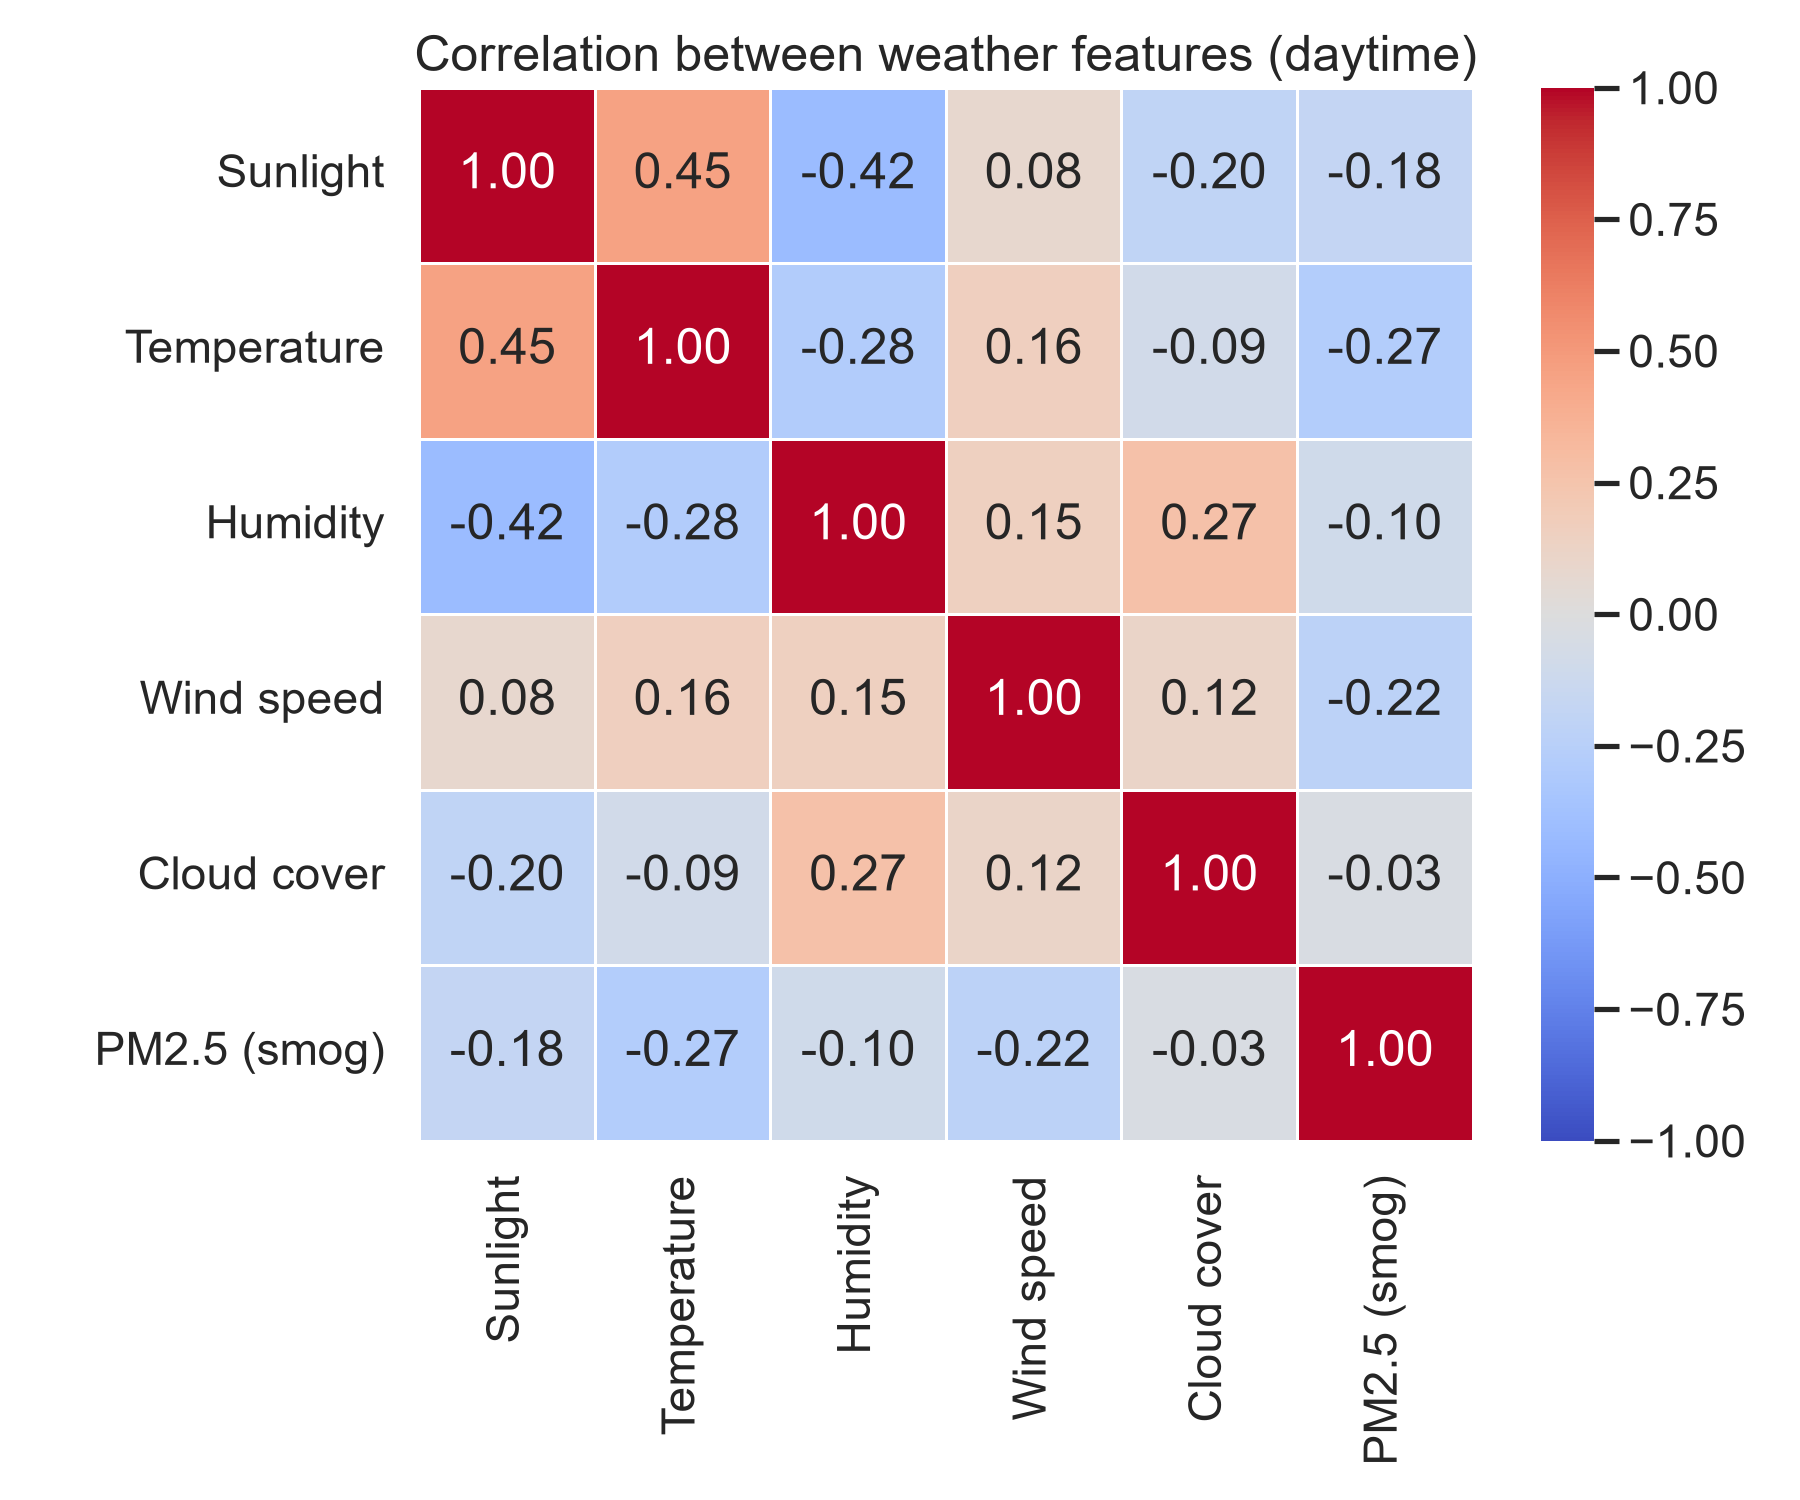
\includegraphics[width=0.72\textwidth]{02_correlation_heatmap.png}
\caption{Correlation between the weather features for daytime hours.}
\label{fig:corr}
\end{figure}

\subsection{Sunlight and panel output}
Figure~\ref{fig:output} compares sunlight with the DC power produced by the inverters in the Kaggle plant data. The two are almost perfectly linked, with a correlation of r = 0.993 across 68,711 cleaned readings. This confirms that sunlight is the main driver of solar output, so accurate sunlight forecasts will translate directly into accurate generation forecasts.

\begin{figure}[H]
\centering
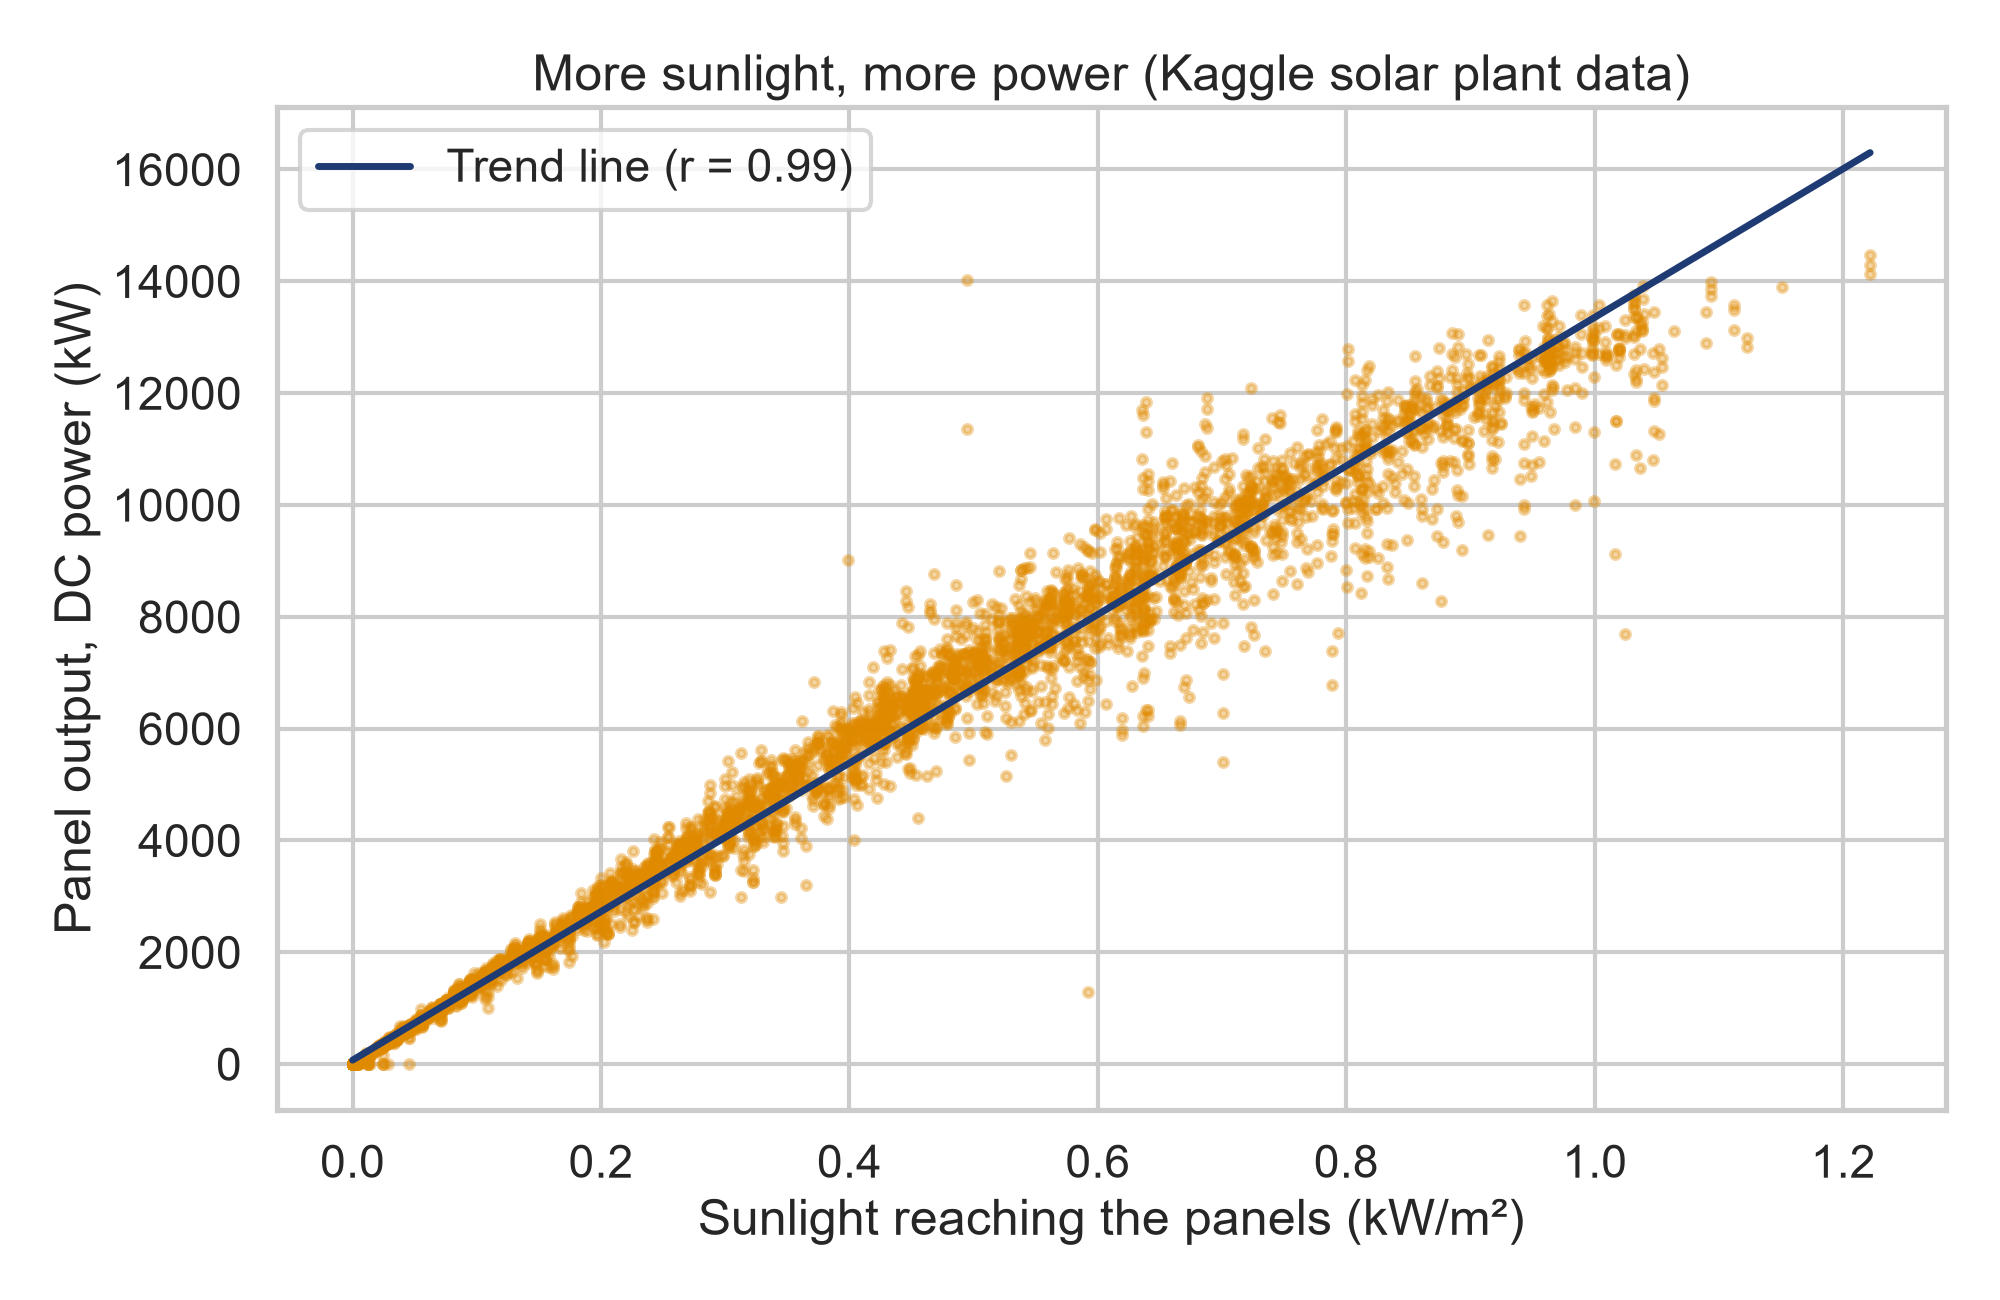
\includegraphics[width=0.8\textwidth]{03_sunlight_vs_output.png}
\caption{Sunlight against panel output (DC power) in the Kaggle solar plant data.}
\label{fig:output}
\end{figure}

\subsection{Cloud cover and sunlight}
The Kaggle plant data does not record cloud cover and comes from a different place and year, so we cannot plot cloud cover against panel output directly. Instead we show the effect in two steps: Figure~\ref{fig:cloud} shows how cloud cover changes sunlight, and Figure~\ref{fig:output} shows how sunlight changes output. For Figure~\ref{fig:cloud} we only use the hours from 11:00 to 13:00, when the sun is highest, so that the effect of the time of day is mostly removed.

Midday sunlight stays fairly steady while cloud cover rises up to about 80\%, and drops clearly under heavy overcast. At 90 to 100\% cloud cover the average is about 490~W/m$^2$, against about 730~W/m$^2$ under clear skies (below 10\% cloud), a fall of 32\%. The correlation between cloud cover and midday sunlight is moderate ($r = -0.41$). The wide spread inside each band has two main causes: the sun sits lower in winter than in summer even at midday, and cloud cover and sunlight come from two different models (Open-Meteo and NASA), which do not always agree. For the project this means cloud cover is a useful but imperfect input, and it supports using several weather inputs together instead of a single formula.

\begin{figure}[H]
\centering
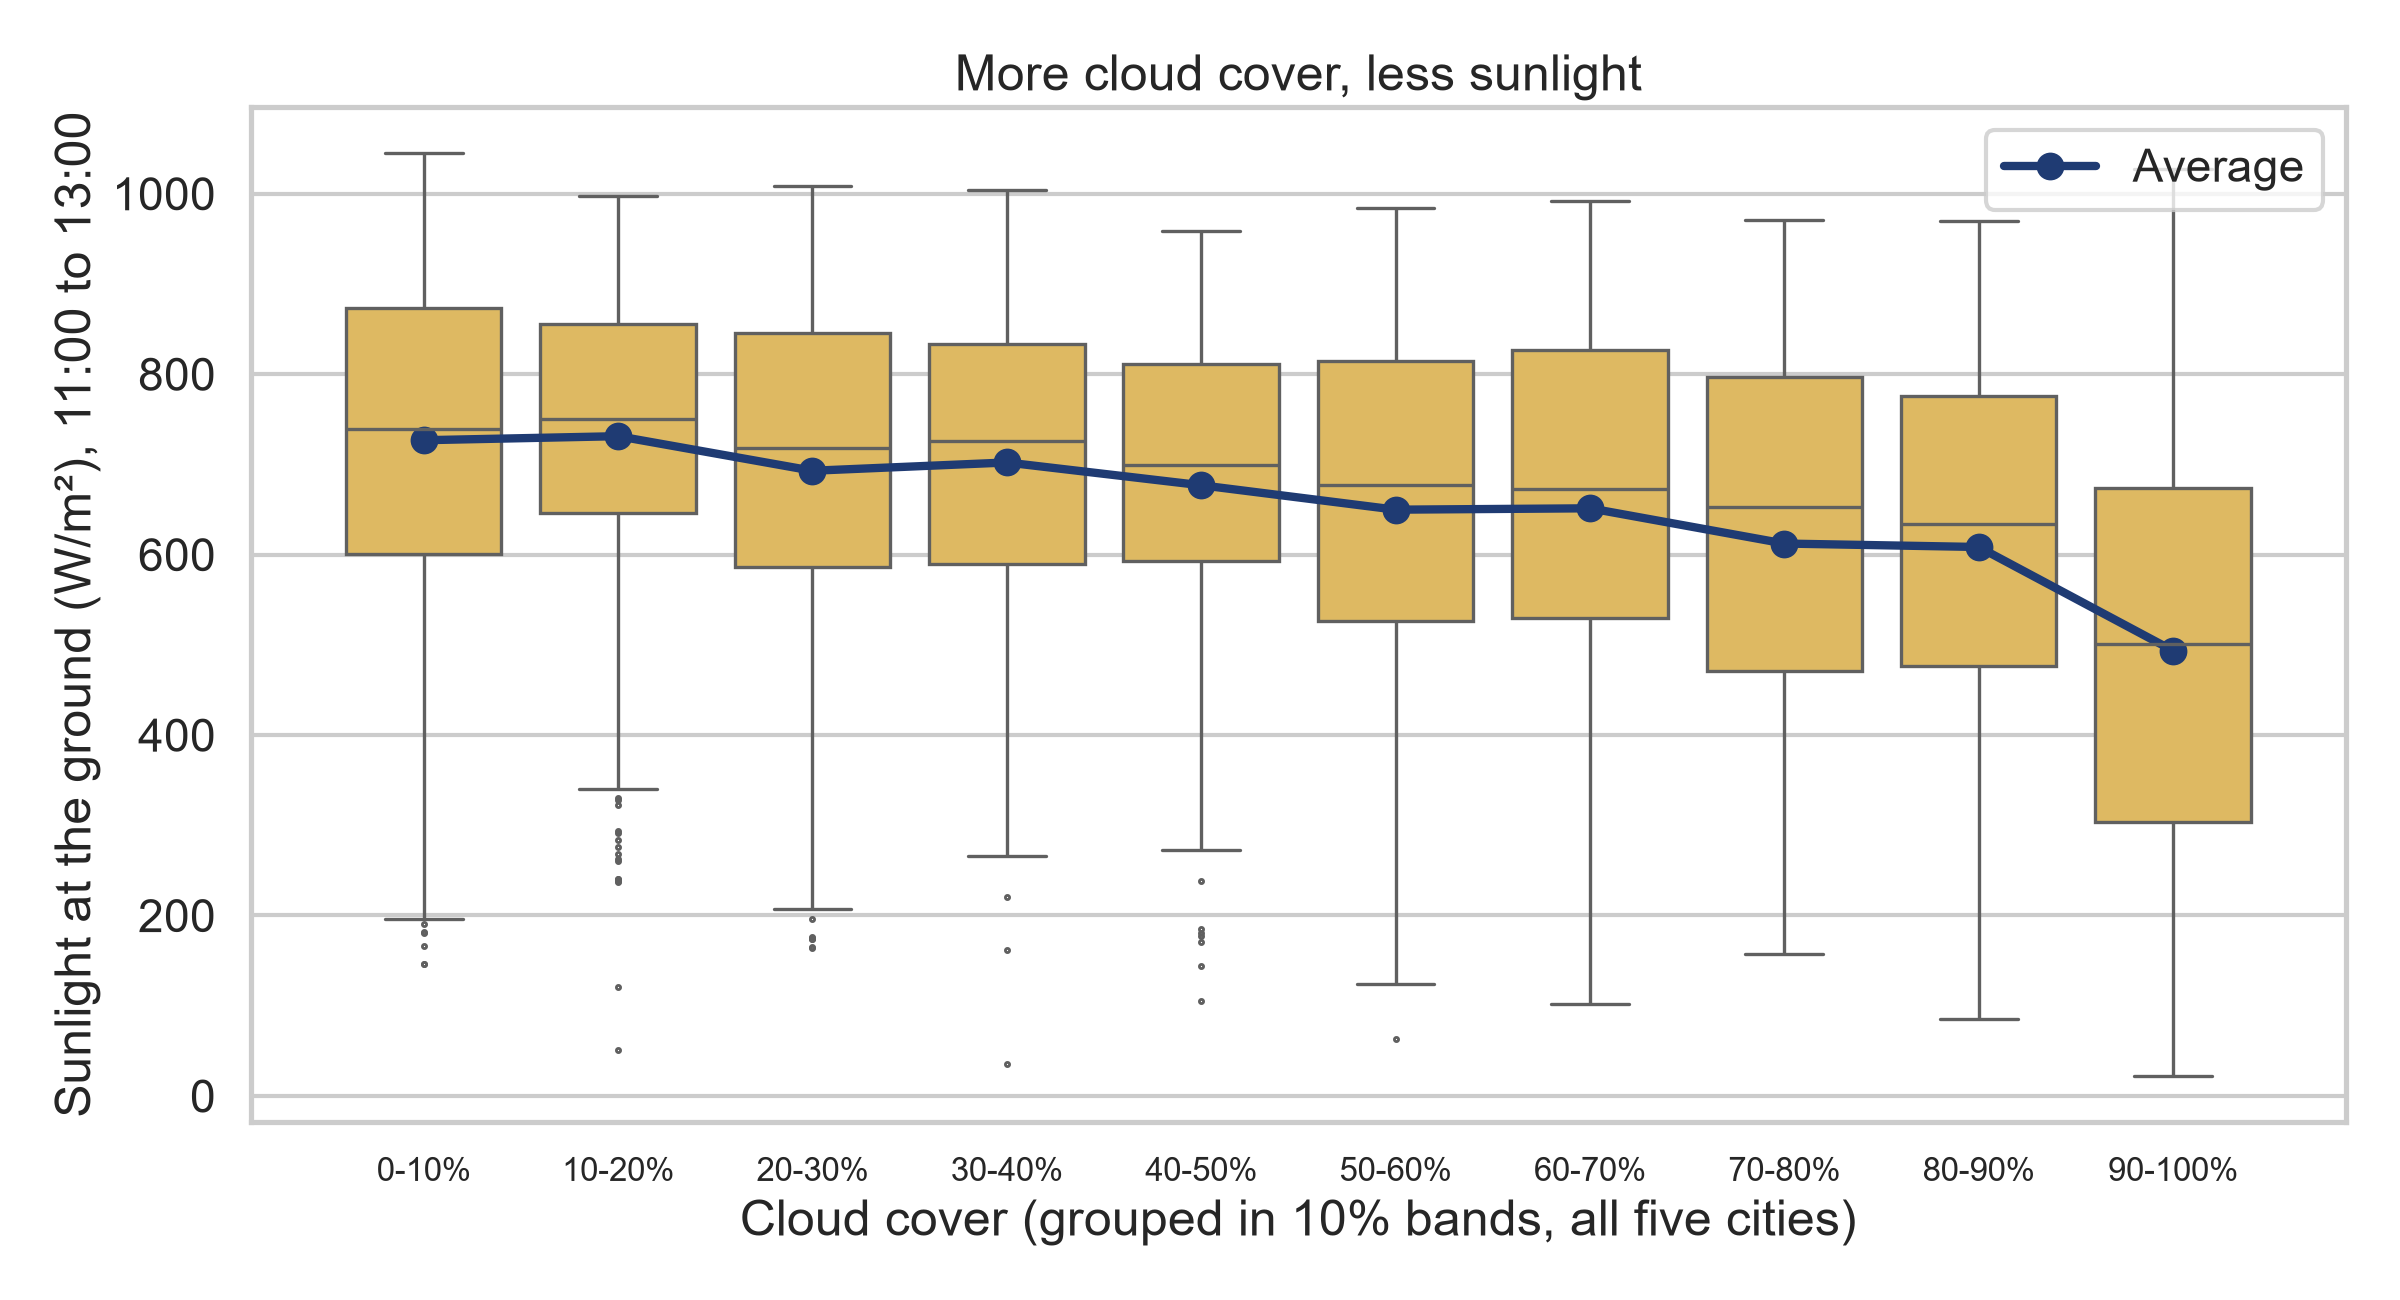
\includegraphics[width=0.88\textwidth]{04_cloud_cover_vs_sunlight.png}
\caption{Midday sunlight (11:00 to 13:00) for each 10\% band of cloud cover, all five cities. The line connects the band averages.}
\label{fig:cloud}
\end{figure}

\subsection{Missing values}
Figure~\ref{fig:missing} shows the share of missing values in each raw weather column before cleaning. We found none in the NASA POWER columns (after treating the $-999$ code as missing) or in the Open-Meteo columns, so none of these values had to be filled in. The cleaning of the Kaggle plant data (faulty inverters and invalid night readings) is described in the Data Cleaning section.

\begin{figure}[H]
\centering
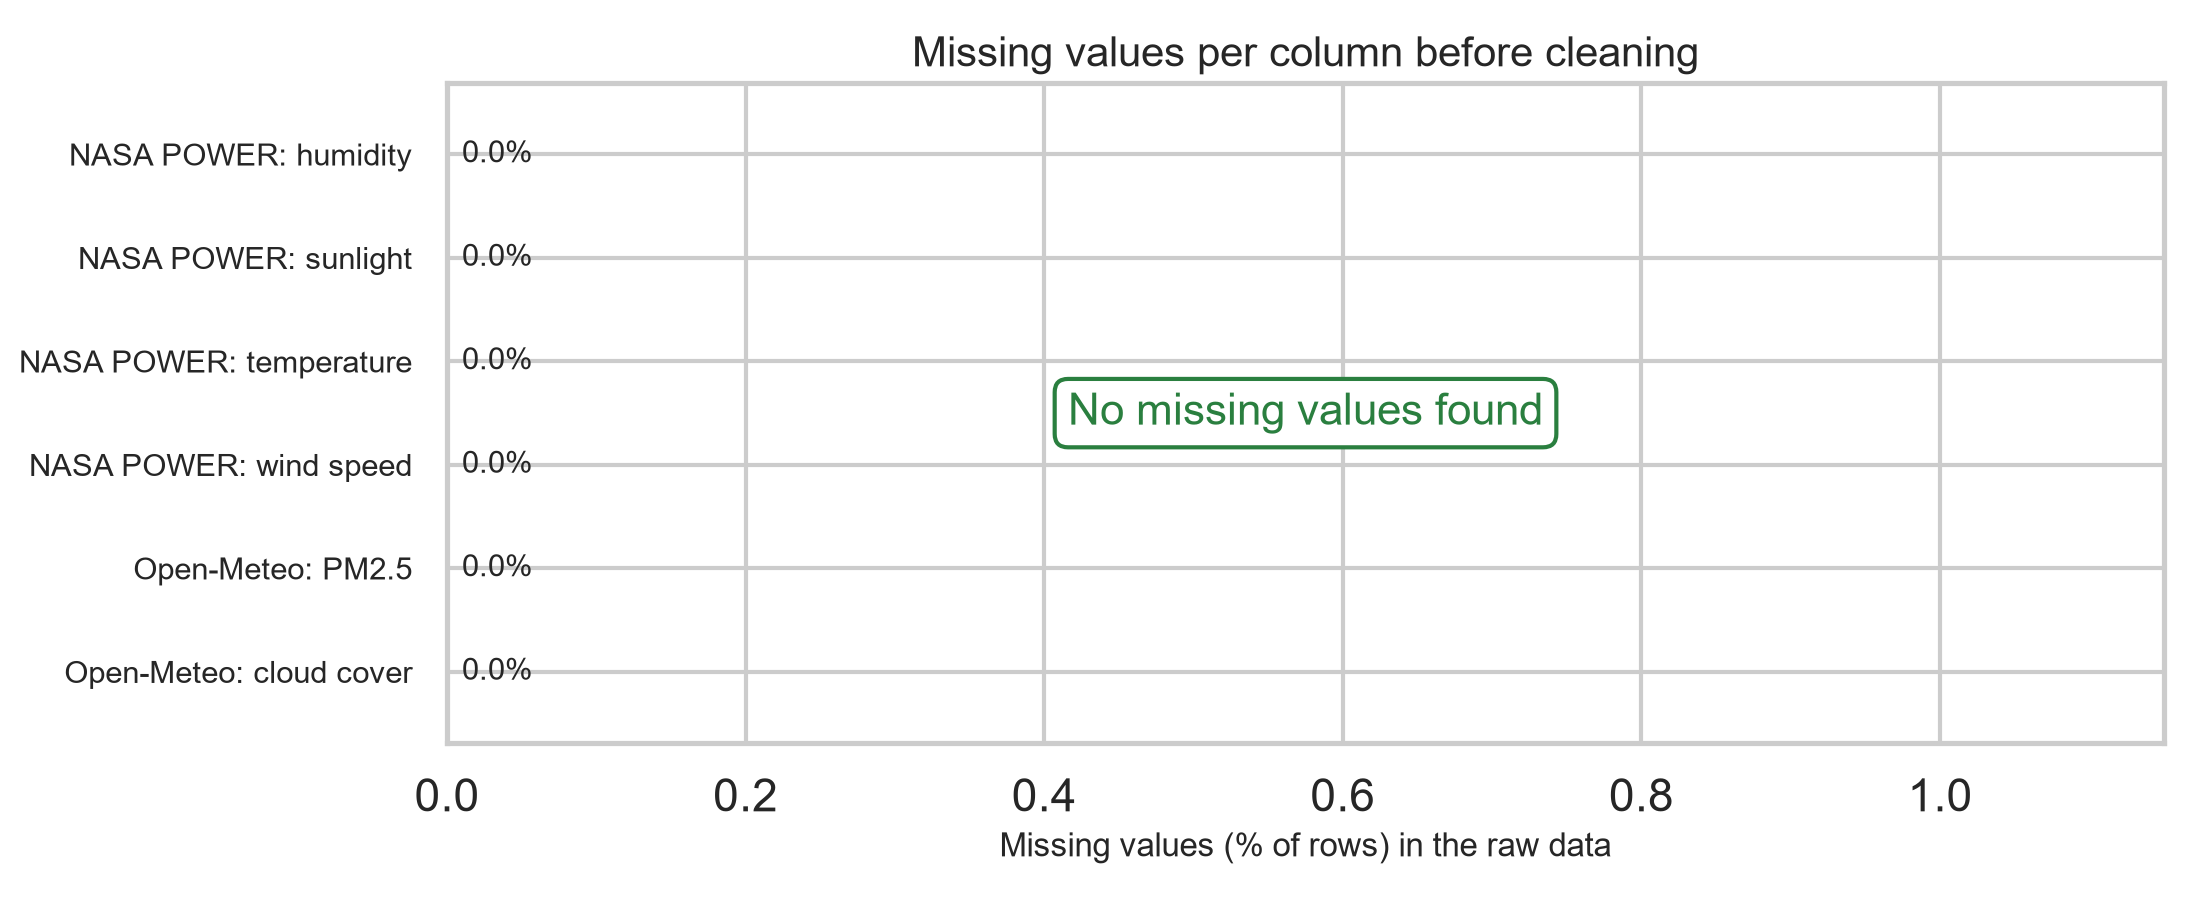
\includegraphics[width=0.85\textwidth]{05_missing_values.png}
\caption{Missing values per column in the raw data.}
\label{fig:missing}
\end{figure}

\subsection{What the analysis tells us}
Sunlight is the main driver of output and varies strongly by month and city. Temperature, humidity, cloud cover and smog each have a smaller effect, and they act together, which supports using a machine learning model with all of them as inputs. The city must also be an input, and this is why we one hot encode it.

\section{Next Steps}
With the data pipeline complete, the next stage of the project has four parts. First, we will train machine learning models that predict hourly solar output from the weather features and the city, and evaluate them on a held-out test set. Second, we will compare these models against a simple physics-based baseline, so that we can show how much the data-driven approach improves on a fixed formula. Third, we will build a web app where a user selects a city and system size and sees the forecast output, expected savings and nearby retailers from \texttt{data/retailers.csv}. Finally, we will add a chatbot that answers common questions about rooftop solar in Pakistan.

\end{document}